\chapter{Advanced Posters}

This chapter expands on the \texttt{poster} doctype overview from
Chapter~\ref{ch:visual} with detailed customization, layout strategies,
and integration with OmniLaTeX's TikZ and plotting libraries.

\section{Design Philosophy}

OmniLaTeX posters use \texttt{scrartcl} with an A1 landscape layout
(841\,mm $\times$ 594\,mm).  Unlike dedicated poster classes such as
\texttt{beamerposter}, the OmniLaTeX approach:

\begin{itemize}
    \item Provides the same typography, bibliography, and code listing
          infrastructure as all other doctypes.
    \item Uses standard \texttt{multicol} for column layout rather than
          a custom grid system.
    \item Defines poster-specific tcolorbox environments for titled and
          untitled content blocks.
    \item Supports all OmniLaTeX features including glossaries, minted
          code listings, and institution colour schemes.
\end{itemize}

The poster profile is defined in
\texttt{config/document-types/poster.sty}.

\section{Layout Configuration}

The doctype applies these settings automatically:

\begin{table}[htbp]
    \centering
    \caption{Poster doctype defaults}
    \label{tab:poster-defaults}
    \begin{tabular}{@{} l l @{}}
        \toprule
        \textbf{Setting} & \textbf{Value} \\
        \midrule
        Font size      & 20\,pt \\
        Font mode      & Sans-serif \\
        Paper size     & A1 landscape (841\,mm $\times$ 594\,mm) \\
        KOMA \texttt{DIV} & 20 \\
        Line spacing   & Single \\
        Page style     & Empty \\
        Section depth  & 0 (no section numbers) \\
        TOC depth      & 0 \\
        Colour mode    & Full colour \\
        \bottomrule
    \end{tabular}
\end{table}

Override paper dimensions for different conference requirements:

\begin{minted}{latex}
% A0 landscape (1189mm x 841mm)
\AtBeginDocument{%
    \setlength{\paperwidth}{1189mm}%
    \setlength{\paperheight}{841mm}%
}

% A2 portrait (420mm x 594mm)
\AtBeginDocument{%
    \setlength{\paperwidth}{420mm}%
    \setlength{\paperheight}{594mm}%
}
\end{minted}

\section{Title Page}

The \texttt{\textbackslash maketitle} override renders the title in 60\,pt
bold, the author list in \texttt{\textbackslash LARGE}, and the date in
\texttt{\textbackslash Large}, all centred.  No decorative bars or TikZ
overlays are drawn.

\begin{minted}{latex}
\documentclass[doctype=poster, institution=none]{../../omnilatex}
\title{OmniLaTeX: A Universal Document Template}
\author{Jane Doe, John Smith}
\date{International Conference on Document Engineering, 2026}
\begin{document}
\maketitle
% Poster content follows
\end{document}
\end{minted}

The title page adds 8\,mm of vertical space after the date block before
content begins.

\section{Poster Block Environments}

Two tcolorbox environments are defined:

\subsection{posterblock}

\begin{minted}{latex}
\begin{posterblock}[Section Title]
    Content goes here.  Supports all standard \LaTeX{} commands,
    including itemize, enumerate, math, and figures.
\end{posterblock}
\end{minted}

Default styling:

\begin{itemize}
    \item White background
    \item Frame colour: \texttt{black!70}
    \item Title text: white on \texttt{black!70} background
    \item Title font: \texttt{\textbackslash bfseries\textbackslash Large}
    \item Rounded corners: 3\,mm
    \item Box rule: 1.5\,pt
    \item Inner padding: 8\,mm all sides
\end{itemize}

\subsection{posterblocknotitle}

\begin{minted}{latex}
\begin{posterblocknotitle}
    \centering
    % Embedded figure or TikZ diagram
    \includegraphics[width=\textwidth]{results-chart}
\end{posterblocknotitle}
\end{minted}

Same styling as \texttt{posterblock} but without the title bar.  Useful for
nesting figures inside a titled block:

\begin{minted}{latex}
\begin{posterblock}[Results]
    Our model achieves 95\% accuracy after 30 epochs.

    \begin{posterblocknotitle}
        \centering
        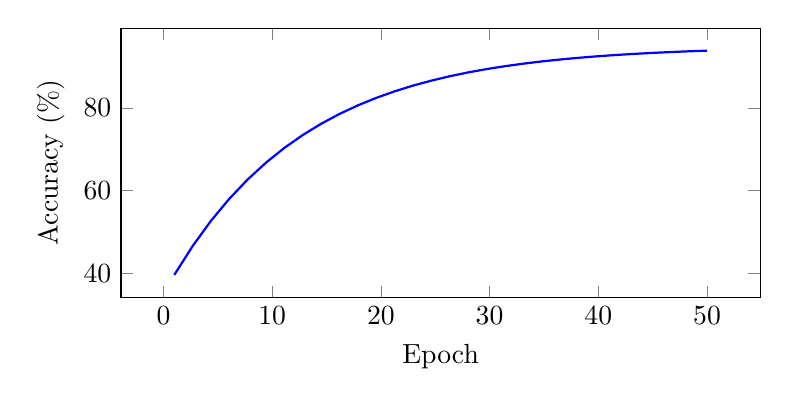
\begin{tikzpicture}
            \begin{axis}[
                width=0.8\textwidth,
                height=50mm,
                xlabel={Epoch},
                ylabel={Accuracy (\%)},
            ]
                \addplot[blue, thick, domain=1:50, samples=30]
                    {95 - 60*exp(-0.08*x)};
            \end{axis}
        \end{tikzpicture}
    \end{posterblocknotitle}
\end{posterblock}
\end{minted}

\section{Customising Block Styles}

Since both environments are standard tcolorbox definitions, you can override
them in \texttt{config/document-settings.sty}:

\begin{minted}{latex}
% Redefine posterblock with institution colours
\renewtcolorbox{posterblock}[1][]{%
    enhanced,
    colback=white,
    colframe=universityprimary,
    coltitle=white,
    fonttitle=\bfseries\Large,
    title=#1,
    arc=3mm,
    boxrule=1.5pt,
    top=8mm, bottom=8mm, left=8mm, right=8mm,
}
\end{minted}

This replaces the default \texttt{black!70} frame with the institution's
primary colour.

\section{Layout Helpers}

\subsection{posterwidth}

The \texttt{\textbackslash posterwidth} command provides a consistent width
for blocks:

\begin{minted}{latex}
\begin{posterblock}[Introduction]
    % This block automatically uses 0.9\textwidth internally
    % via the \posterwidth length if you reference it:
    Content with \texttt{\textbackslash posterwidth} = 0.9\textbackslash textwidth.
\end{posterblock}
\end{minted}

The length is defined as \texttt{\textbackslash providecommand}, so it can be
redefined:

\begin{minted}{latex}
\renewcommand{\posterwidth}{0.95\textwidth}
\end{minted}

\subsection{Column Breaks}

Use \texttt{\textbackslash columnbreak} inside \texttt{multicols} to force
content to the next column:

\begin{minted}{latex}
\begin{multicols}{3}
    \begin{posterblock}[Introduction]
        First block in column 1.
    \end{posterblock}
    \begin{posterblock}[Methods]
        Second block in column 1.
    \end{posterblock}

    \columnbreak  % Force to column 2

    \begin{posterblock}[Results]
        First block in column 2.
    \end{posterblock}

    \columnbreak  % Force to column 3

    \begin{posterblock}[Conclusion]
        First block in column 3.
    \end{posterblock}
\end{multicols}
\end{minted}

\section{Multi-Column Layout Strategy}

The \texttt{multicol} package handles column balancing automatically, but
posters typically need manual control.  Use these strategies:

\begin{minted}{latex}
\begin{multicols}{3}

    % === Column 1 ===
    \begin{posterblock}[Introduction]
        Background and motivation\ldots
    \end{posterblock}
    \begin{posterblock}[Objectives]
        Research questions\ldots
    \end{posterblock}

    \columnbreak

    % === Column 2 ===
    \begin{posterblock}[Methods]
        Experimental setup\ldots
    \end{posterblock}
    \begin{posterblock}[Results]
        Key findings with embedded chart\ldots
        \begin{posterblocknotitle}
            \centering
            % pgfplots or TikZ figure
        \end{posterblocknotitle}
    \end{posterblock}

    \columnbreak

    % === Column 3 ===
    \begin{posterblock}[Discussion]
        Interpretation\ldots
    \end{posterblock}
    \begin{posterblock}[References]
        \small
        \begin{enumerate}
            \item Author, \textit{Title}, Journal, Year.
        \end{enumerate}
    \end{posterblock}

\end{multicols}
\end{minted}

For two-column posters, use \texttt{\textbackslash begin\{multicols\}\{2\}}
and adjust block widths if needed.

\section{Embedding TikZ Diagrams}

Posters often include architecture diagrams or flowcharts.  Use
\texttt{posterblocknotitle} as a container:

\begin{minted}{latex}
\begin{posterblock}[System Architecture]
    \begin{posterblocknotitle}
        \centering
        \begin{tikzpicture}[
            box/.style={draw, thick, rounded corners,
                minimum height=10mm, minimum width=22mm,
                fill=universityprimary!10, font=\small},
            arr/.style={->, thick, >=stealth},
            node distance=10mm,
        ]
            \node[box] (input) {Input Data};
            \node[box, below=of input] (proc) {Processing};
            \node[box, below left=of proc] (model) {Model};
            \node[box, below right=of proc] (eval) {Evaluation};
            \node[box, below=of proc] (output) {Output};

            \draw[arr] (input) -- (proc);
            \draw[arr] (proc) -- (model);
            \draw[arr] (proc) -- (eval);
            \draw[arr] (model) -- (output);
            \draw[arr] (eval) -- (output);
        \end{tikzpicture}
    \end{posterblocknotitle}
\end{posterblock}
\end{minted}

Use \texttt{universityprimary!10} for fill colours to maintain visual
consistency with the header.

\section{Embedding pgfplots Charts}

Combine pgfplots with \texttt{posterblocknotitle} for data visualisation:

\begin{minted}{latex}
\begin{posterblock}[Experimental Results]
    Accuracy improves with training epochs.

    \begin{posterblocknotitle}
        \centering
        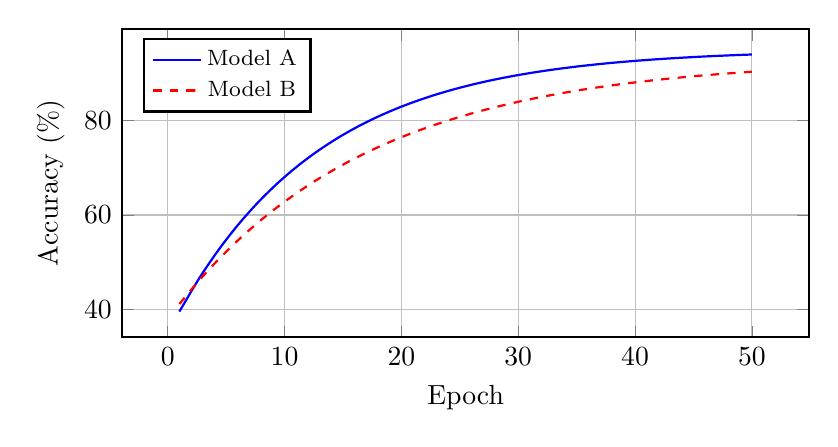
\begin{tikzpicture}
            \begin{axis}[
                width=0.85\textwidth,
                height=55mm,
                xlabel={Epoch},
                ylabel={Accuracy (\%)},
                legend style={font=\footnotesize,
                    at={(0.03,0.97)}, anchor=north west},
                grid=major,
                thick,
            ]
                \addplot[blue, thick, smooth, domain=1:50, samples=30]
                    {95 - 60*exp(-0.08*x)};
                \addlegendentry{Model A}

                \addplot[red, thick, dashed, smooth, domain=1:50, samples=30]
                    {93 - 55*exp(-0.06*x)};
                \addlegendentry{Model B}
            \end{axis}
        \end{tikzpicture}
    \end{posterblocknotitle}
\end{posterblock}
\end{minted}

Set \texttt{width} relative to \texttt{\textbackslash textwidth} to scale
with column width.  Heights between 45\,mm and 60\,mm work well for A1
posters.

\section{Code Listings on Posters}

The \texttt{minted} package works inside poster blocks:

\begin{minted}{latex}
\begin{posterblock}[Algorithm]
    \begin{posterblocknotitle}
        \begin{minted}[fontsize=\footnotesize]{python}
def train(model, data, epochs=50):
    for epoch in range(epochs):
        loss = model.step(data)
        print(f"Epoch {epoch}: loss={loss:.4f}")
    return model
        \end{minted}
    \end{posterblocknotitle}
\end{posterblock}
\end{minted}

Use \texttt{fontsize=\textbackslash footnotesize} or
\texttt{fontsize=\textbackslash small} to fit code within poster blocks.

\section{Building Posters}

\begin{minted}{bash}
# Via Docker
docker run --rm --entrypoint "" \
    -v "$PWD:/workspace" \
    ghcr.io/wyattau/omnilatex:latest \
    python3 build.py --mode prod --force build-example poster

# Via Nix
nix develop .# --command python3 build.py --mode prod build-example poster
\end{minted}

Poster compilation is slower than other doctypes due to the large page size
and TikZ/pgfplots rendering.  Allow 30--60 seconds for complex posters.

\section{Institution Integration}

Load an institution config to apply its colour scheme:

\begin{minted}{latex}
\documentclass[
    doctype=poster,
    institution=tuhh,
    enabletikz=true,
    enableengineering=true,
]{../../omnilatex}
\end{minted}

The institution's \texttt{universityprimary} and \texttt{universitysecondary}
colours become available for use in poster blocks and TikZ diagrams.  You
can reference them directly:

\begin{minted}{latex}
\begin{posterblock}[Introduction]
    % Use institution colour for emphasis
    \textcolor{universityprimary}{\textbf{Key insight:}}
    Our approach reduces compile time by 40\%.
\end{posterblock}
\end{minted}

\section{Common Patterns}

\subsection{QR Code for Digital Supplement}

Include a QR code linking to a repository or supplementary material:

\begin{minted}{latex}
\usepackage{qrcode}

\begin{posterblock}[Online Resources]
    \begin{posterblocknotitle}
        \centering
        \qrcode[height=30mm]{https://github.com/WyattAu/OmniLaTeX-template}\\[4mm]
        \small\texttt{github.com/WyattAu/OmniLaTeX-template}
    \end{posterblocknotitle}
\end{posterblock}
\end{minted}

\subsection{Acknowledgements Section}

Use a narrow block at the bottom of the final column:

\begin{minted}{latex}
\begin{posterblock}[Acknowledgements]
    \small
    This work was supported by the National Science Foundation
    (Grant \#12345).  We thank our colleagues for valuable feedback.
\end{posterblock}
\end{minted}

\subsection{Numbered References}

For conferences requiring numbered references:

\begin{minted}{latex}
\begin{posterblock}[References]
    \small
    \begin{enumerate}
        \item A.\ Author, B.\ Author.
              \textit{Title of Paper}.
              Journal Name, 2025.
        \item C.\ Author.
              \textit{Another Title}.
              Proceedings of Conference, 2026.
    \end{enumerate}
\end{posterblock}
\end{minted}

For biblatex integration, use the standard
\texttt{\textbackslash printbibliography} command with a
\texttt{refsection} if you need poster-specific references.
